\problemname{Skidor}
Lille Fredrik vill bygga ett så högt torn som möjligt med sina N klossar. Alla klossar är rätblock med en kvadratisk botten, och ett torn är en mängd med klossar som är staplade direkt ovanpå varandra (det får inte ligga två klossar bredvid varandra). För att tornet inte ska bli instabilt och rasa måste varje kloss bredd (alltså sidan på den kvadratiska botten den står på) alltid vara strikt mindre än bredden av klossen den står på. Alltså byggs tornet med de bredaste klossarna i botten, och smalare klossar ju högre upp man kommer. Dessutom måste även varje kloss vara minst lika högt som klossen nedanför, för att tornet ska bli snyggt. Hjälp Fredrik att räkna ut hur högt torn han maximalt kan bygga.


\section*{Indata}
Den första raden innehåller ett heltal $N$, antalet klossar Fredrik har. Därefter följer $N$ rader, en för varje kloss. På den $i$:te av dessa rader står talen $W_i$ och $H_i$, $1 \leq W_i,H_i \leq 10^9$.

\begin{wrapfigure}{R}{0.3\textwidth}
\centering
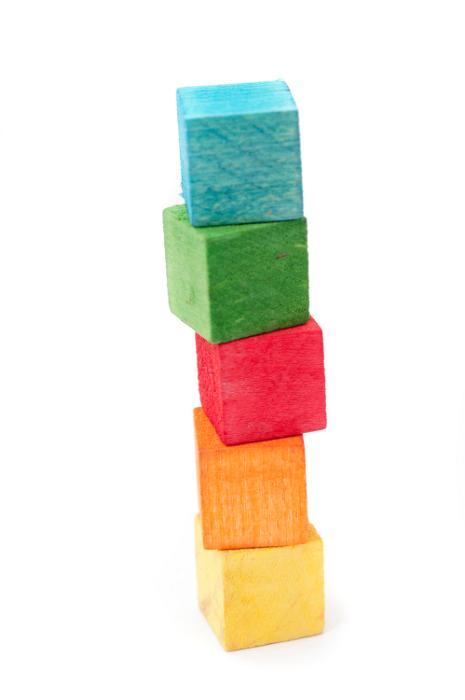
\includegraphics[width=0.25\textwidth]{klossar.jpg}
\caption{\label{fig:frog1}This is a figure caption.}
\end{wrapfigure}

\section*{Output}
Skriv ut en rad med ett heltal: den maximala höjden som Fredrik kan bygga. Detta tal garanteras vara mindre än $10^9$.
\section*{Poängsättning}
Din lösning kommer att testas på en mängd testfallsgrupper. För att få poäng för en grupp så måste du klara alla testfall i gruppen.
\begin{tabular}{|l|l|l|}
\hline
Grupp & Poängvärde & Gränser \\ \hline
 1     & 21         &  $0 \leq H_i \leq 1$ \\ \hline
 2     & 36         &  $N \leq 50$ \\ \hline
 3     & 27         &  $N \leq 300$ \\ \hline
 4     & 16         &  $N \leq 1000$ \\ \hline
\end{tabular}
